\documentclass{beamer}


\usepackage{amsmath}
\usepackage[style=alphabetic,url=true]{biblatex}
\usepackage{environ}
\usepackage{geometry}
\usepackage{graphicx}
\usepackage{tikz}
\usepackage[T2A]{fontenc}
\usepackage[utf8]{inputenc}
\usepackage[cache=false]{minted}
\usepackage{amsmath}
\usepackage{amsfonts}
\usepackage{amssymb}
\usepackage{calrsfs}
\usepackage{animate}
\usepackage{xmpmulti}


% \usetheme{Bergen}

\usecolortheme{beaver}

\setbeamertemplate{itemize item}[circle]
\setbeamertemplate{itemize subitem}{--}
\addtobeamertemplate{navigation symbols}{}{
  \usebeamerfont{footline}%
  \usebeamercolor[fg]{footline}%
  \hspace{1em}%
  \insertframenumber/\inserttotalframenumber
}
\graphicspath{ {./graphics/} }
\setminted[Python]{
  fontsize=\tiny
}
\setminted[Lisp]{
  fontsize=\tiny
}
\BeforeBeginEnvironment{minted}{\medskip}
\AfterEndEnvironment{minted}{\medskip}
\usetikzlibrary{matrix}
\tikzset{
  stack/.style={
    matrix of nodes,
    nodes={
      fill=lightgray,draw,text=black,font=\sffamily\bfseries,
      text height=11pt,text depth=3pt,baseline=center, minimum width=1cm
    },
    column sep=-\pgflinewidth/2
  }
}

\title{
  Біткоїн та криптовалютні технології \\
  Лекція 9: Масштабування Біткоїна 1/2
}

\author{Юрій Жикін}
\date{21 квітня, 2025}

\begin{document}

\frame{\titlepage}

\begin{frame}
  \frametitle{Пропускна здатність транзакцій}
  \begin{itemize}
  \item Блок кожні 10 хвилин (600 секунд).
  \item Середній розмір кожного блока - 1.5 Мб.
  \item Середній розмір транзакції - 500 байтів.
  \item Пропускна здатність
    $$T = \frac{1.5 * 1024 * 1024}{500 * 600} \approx 5 \text{ т/с}$$
  \item Пропускна здатність Visa - приблизно 1700 т/с.
  \end{itemize}
\end{frame}

\begin{frame}
  \frametitle{Пропозиції щодо масштабування пропускної здатності}
  \begin{itemize}
  \item \textbf{Збільшення розміру блока} - збільшення централізації; поточна
    швидкість зростання розміру ланцюга - 80 Гб/рік.
  \item \textbf{Збільшення частоти створення блоків} - збільшення централізації,
    менша стабільність мережі.
  \item \textbf{Оптимізація структури транзакцій} - обмежені можливості.
  \item \textbf{Протоколи другого рівня} - єдиний практичний підхід?
  \end{itemize}
\end{frame}

\begin{frame}
  \frametitle{Оптимізація структури транзакцій}
  \begin{itemize}
  \item \textbf{SegWit} (``відділений свідок'').
  \item \textbf{Підписи Шнорра}.
  \item \textbf{Меркелізовані абстрактні синтаксичні дерева} (\textbf{MAST}).
  \item \textbf{Taproot} (\textbf{Schnorr} + \textbf{MAST}).
  \end{itemize}
\end{frame}

\begin{frame}
  \frametitle{SegWit 1/4}
  \begin{itemize}
  \item Оновлення протоколу, яке було активоване у 2017 році та вирішило
    наступні проблеми:
    \begin{itemize}
    \item \textbf{проблема модифікації транзакцій} - протокол дозволяв внесення
      змін до транзакції так, що змінюється її ідентифікатор, при цьому підпис
      залишається дійсним;
    \item \textbf{оптимізація використання місця у блоці} - усунення потреби
      зберігати великий скрипт відмикання в блоці - його перенесено в окрему
      структуру \textbf{Witness};
    \item \textbf{майбутні оновлення} - SegWit запровадив простий і чіткий
      механізм оновлення транзакційного протоколу через \textbf{м'які
        розгалуження} (softforks).
    \end{itemize}
  \end{itemize}
\end{frame}

\begin{frame}
  \frametitle{SegWit 2/4}
  \begin{itemize}
  \item SegWit продовжив ідею P2SH (BIP-0016) - додаткові правила перевірки
    скриптів активуються при розпізнаванні певного патерну в скрипті.
  \item Основні компоненти транзакції тепер - це \textbf{входи}, \textbf{виходи}
    та \textbf{свідки} (\textbf{witnesses}) (один \textbf{свідок} на кожен
    \textbf{вхід}).
  \item Для кожного входу транзакції, якщо \textbf{скрипт замикання}, який
    \textit{виконується}, виглядає як патерн \textbf{програми-свідка}:
    \begin{itemize}
    \item декодується відповідний \textbf{свідок},
    \item перевіряється, що \textbf{програма-відмикання} відповідає хешу
      \textbf{свідка},
    \item \textbf{свідок} інтерпретується як \textbf{скрипт відмикання}.
    \end{itemize}
  \end{itemize}
\end{frame}

\begin{frame}
  \frametitle{SegWit 3/4}
  \small
  \begin{itemize}
  \item \textbf{P2WPKH} - оплата за хеш публічного ключа свідчення
    (pay-to-witness-public-key-hash) \break
    \begin{tabular}{rl}
      Замикання: &\tiny\mintinline[bgcolor=lightgray]{Lisp}{0 <20-байтовий-хеш-ключа>;} \\
      Відмикання: &\tiny\mintinline[bgcolor=lightgray]{Lisp}{;} \\
      Свідок: &\tiny\mintinline[bgcolor=lightgray]{Lisp}{<підпис> <публічний ключ>} \\
    \end{tabular}
  \item \textbf{P2WSH} - оплата за хеш скрипта свідчення (pay-to-witness-script-hash)
    \break
    \begin{tabular}{rl}
      Замикання: &\tiny\mintinline[bgcolor=lightgray]{Lisp}{0 <32-байтовий-хеш-ключа>;} \\
      Відмикання: &\tiny\mintinline[bgcolor=lightgray]{Lisp}{;} \\
      Свідок: &\tiny\mintinline[bgcolor=lightgray]{Lisp}{0 <підпис1> 1 <пубключ1> <пубключ2> 2 CHECKMULTISIG} \\
    \end{tabular}
  \item \textbf{P2SH-P2WPKH} - P2WPKH вкладений у P2SH за BIP16
    \break
    \begin{tabular}{rl}
      Замикання: &\tiny\mintinline[bgcolor=lightgray]{Lisp}{HASH160 <20-байтовий-хеш-скрипта> EQUAL;} \\
      Відмикання: &\tiny\mintinline[bgcolor=lightgray]{Lisp}{<0 <20-байтовий-хеш-ключа>>;} \\
      Свідок: &\tiny\mintinline[bgcolor=lightgray]{Lisp}{<підпис> <публічний ключ>} \\
    \end{tabular}
  \item \textbf{P2SH-P2WSH} - P2WSH вкладений у P2SH за BIP16
    \break
    \begin{tabular}{rl}
      Замикання: &\tiny\mintinline[bgcolor=lightgray]{Lisp}{HASH160 <20-байтовий-хеш> EQUAL;} \\
      Відмикання: &\tiny\mintinline[bgcolor=lightgray]{Lisp}{<0 <32-байтовий-хеш-ключа>>;} \\
      Свідок: &\tiny\mintinline[bgcolor=lightgray]{Lisp}{0 <підпис1> 1 <пубключ1> <пубключ2> 2 CHECKMULTISIG} \\
    \end{tabular}
  \end{itemize}
\end{frame}

\begin{frame}
  \frametitle{SegWit 4/4}
  \small
  \begin{itemize}
  \item Свідки включаються в ланцюг через \textbf{кореневий хеш}
    (\textbf{witness root hash}), який записується в \textbf{скрипті замикання}
    породжуючої транзакції.
  \item \textbf{Кореневий хеш} - це \textit{корінь мерклевого дерева}
    побудованого з \textbf{wtxid}:
    \break
    \begin{tabular}{rl}
      \mintinline{Lisp}{txid}: &\tiny\mintinline[bgcolor=lightgray]{Lisp}{[nVersion][txins][txouts][nLockTime]} \\
      \mintinline{Lisp}{wtxid}: &\tiny\mintinline[bgcolor=lightgray]{Lisp}{[nVersion][marker][flag][txins][txouts][witness][nLockTime]} \\
    \end{tabular}
  \item Обмеження на розмір блока ($1,000,000$) змінено наступним чином:
    \begin{itemize}
    \item $BlockWeight$ визначається як $BaseSize * 3 + TotalSize$;
    \item $BaseSize$ - це розмір блока в байтах при оригінальній серіалізації
      транзакцій без будь-яких даних свідків;
    \item $TotalSize$ - це розмір блока в байтах з транзакціями, серіалізованими
      згідно з BIP144, включаючи як базові дані, так і дані свідків;
    \item Нова умова: $BlockWeight \leq 4,000,000$.
    \end{itemize}
  \end{itemize}
\end{frame}

\begin{frame}
  \frametitle{Підписи Шнорра}
  \begin{itemize}
  \item \textbf{Підпис Шнорра} - це альтернативна схема криптографічних
    підписів, яка забезпечує певні властивості, корисні для Біткоїн-системи,
    зокрема, \textbf{лінійність}, що дозволяє об'єднувати ключі та підписи:
    \begin{align*}
      &key_x = key_1 + key_2 + \dots + key_n \\
      &sig_x = sig_1 + sig_2 + \dots + sig_n \\
    \end{align*}
  \end{itemize}
\end{frame}

\begin{frame}
  \frametitle{MAST і Taproot}
  \begin{itemize}
  \item \textbf{Меркелізовані абстрактні синтаксичні дерева} (\textbf{MAST}) -
    це спосіб підтримки великих і складних скриптів шляхом побудови з них
    \textit{мерклевого дерева} і відмикання за допомогою розкриття лише
    потрібного \textbf{шляху у дереві}, що підвищує конфіденційність.
    \begin{center}
      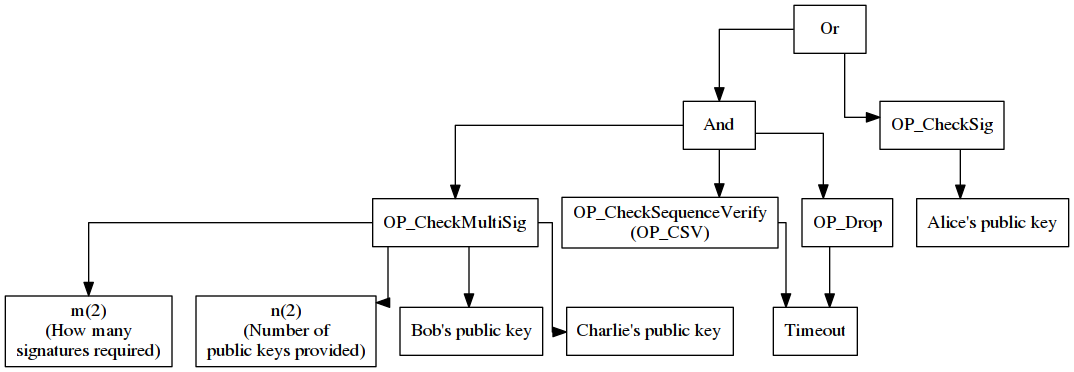
\includegraphics[width=0.8\textwidth]{mast}
    \end{center}
  \item І \textbf{підписи Шнорра}, і варіант \textbf{MAST} є частиною м’якого
    розгалуження \textbf{Taproot}, який було активовано в основній мережі 14
    листопада 2021 року.
  \end{itemize}
\end{frame}

\begin{frame}
  \frametitle{Рекомендовані ресурси}
  \begin{itemize}
  \item \textbf{Bitcoin: A Work in Progress}
    \begin{itemize}
    \item книга автора Сьорса Провоста (Sjors Provoost), одного з активних
      розробників Біткоїна
    \item https://btcwip.com
    \end{itemize}
  \end{itemize}
\end{frame}

\begin{frame}
  \frametitle{Кінець}
  \begin{center}
    Дякую за увагу!
  \end{center}
\end{frame}

\end{document}

%%% Local Variables:
%%% mode: latex
%%% TeX-master: t
%%% End:
